%% LyX 2.2.1 created this file.  For more info, see http://www.lyx.org/.
%% Do not edit unless you really know what you are doing.
\documentclass[sigconf,anonymous=false,authordraft=false]{acmart}
\usepackage[latin9]{inputenc}
\usepackage{verbatim}
\usepackage{float}
\usepackage{url}
\usepackage{enumitem}
\usepackage{graphicx}
\usepackage{balance}
\makeatletter
%%%%%%%%%%%%%%%%%%%%%%%%%%%%%% Textclass specific LaTeX commands.
\newlength{\lyxlabelwidth}      % auxiliary length 

%%%%%%%%%%%%%%%%%%%%%%%%%%%%%% User specified LaTeX commands.
%\renewcommand\footnotetextcopyrightpermission[1]{} % removes footnote with conference information in first column
%\pagestyle{plain} % removes running headers


%\makeatletter
%\renewcommand\@formatdoi[1]{\ignorespaces}
%\makeatother


\usepackage{url}
\usepackage{enumitem}
\usepackage{amstext}
\usepackage{graphicx}
\usepackage{booktabs} % For formal tables




\usepackage{subfigure}
\usepackage[ruled,vlined,linesnumbered]{algorithm2e}

\newcommand\varlist{,\makebox[0.8em][c]{.\hfil.\hfil.},} 

% DOI

% ISBN

%Conference
\copyrightyear{2019} 
\acmYear{2019} 
\setcopyright{rightsretained} 
\acmConference[CHIIR '19]{2019 Conference on Human Information Interaction and Retrieval}{March 10--14, 2019}{Glasgow, United Kingdom}
\acmBooktitle{2019 Conference on Human Information Interaction and Retrieval (CHIIR '19), March 10--14, 2019, Glasgow, United Kingdom}
\acmDOI{10.1145/3295750.3298914}
\acmISBN{978-1-4503-6025-8/19/03}







%\acmPrice{15.00}


\settopmatter{printacmref=true}

\fancyhead{}
\settopmatter{printacmref=true, printfolios=false}

\newcommand{\I}{\mathbb{I}}
\newcommand{\N}{\mathcal{N}}
\newcommand{\E}{\mathrm{E}}
\newcommand{\Ind}{\mathrm{\#}}
\renewcommand{\vec}[1]{\mathbf{#1}}
\newcommand{\Sim}{\mathrm{Sim}}
\newcommand{\ExpOneCall}{\text{Exp-}1\text{-Call@}k}
\newcommand{\PLAR}{\text{PLAR}}

\newcommand{\heq}{\hspace{-.5mm} = \hspace{-.5mm}}
\newcommand{\seq}{\hspace{-1mm} = \hspace{-1mm}}



\newcommand{\ExpNCall}[1]{\text{Exp-}#1\text{-Call@}k}
\newcommand{\TlessK}{T_{\!\!\:k\text{-}1}}
\def\argmax{\operatornamewithlimits{\!arg \;\! max\,}}

\makeatother

\begin{document}
%\title{VTF: A Filter Selection-Based Search Tool for Social Network Visualization} 
%\title{VTF: A Visual Filter Selection-Based Search Tool for Social Network} 
%\title{Viz-TSF: A Visual Twitter Search Tool based on the Filtering of Geo-Temporally Coherent Content}
%\title{Viz-TSF: A Visual Twitter Search Tool based on Query-driven Filter Optimization}
%\title{Viz-TIF: A  Query-driven Filter Optimization Tool for Visual Twitter Search}
%\title{Viz-TIF: A  Query-driven F1-Score Optimization Tool for Filtering Information in a Twitter Search Display}
%\title{Viz-TIF: A Tool for Visual Twitter Information Filtering based on F-Score Optimization}
%\title{Viz-TIR: A Tool for Visual Twitter Information Retrieval based on Relevance-driven Clustering Optimization}
\title[Relevance-driven Clustering for Visual Information Retrieval on Twitter]{Relevance-driven Clustering for Visual \\ Information Retrieval on Twitter}



\author{Mohamed Reda Bouadjenek}
%\orcid{1234-5678-9012}
\affiliation{%
  \institution{University of Toronto}
 % \streetaddress{Department of Mechanical and\\ Industrial Engineering}
  \city{Toronto} 
  \state{Ontario} 
   \postcode{M5S 3G8}
  \country{Canada}
}
\email{mrb@mie.utoronto.ca}

\author{Scott Sanner}
\affiliation{%
  \institution{University of Toronto}
 % \streetaddress{Department of Mechanical and\\ Industrial Engineering}
  \city{Toronto} 
  \state{Ontario} 
   \postcode{M5S 3G8}
  \country{Canada}
}
\email{ssanner@mie.utoronto.ca}



\newcommand{\subfour}[1]{\vspace*{0.5mm}{\noindent\bf #1}}  
\newcommand{\subsubfour}[1]{\vspace*{1mm}{\noindent\bf #1}} 
\begin{abstract}
Geo-temporal visualization of Twitter search results is a challenging task since the simultaneous display of all matching tweets would result in a saturated display. 
In such settings, clustering search results can assist users to scan only a few coherent groups of related tweets rather than many individual tweets.  However, in practice, the use of unsupervised clustering methods such as $k$-means does not necessarily guarantee that the clusters themselves are relevant.
Therefore, we develop a novel method of relevance-driven clustering for visual information retrieval to supply users with highly relevant clusters representing different information perspectives of their queries. 
We specifically propose a Visual Twitter Information Retrieval (Viz-TIR) tool % for relevance-driven clustering and ranking of Twitter search results. 
%At the heart of Viz-TIR is 
which based on a fast greedy algorithm that optimizes an approximation of an expected F1-Score metric to generate these clusters.  We demonstrate its effectiveness w.r.t. $k$-means and a baseline method that shows all top matching results on a scenario related to searching natural disasters in US-based Twitter data.  
Our demo shows that Viz-TIR is easy to use and more precise in extracting geo-temporally coherent clusters given search queries in comparison to $k$-means, thus aiding the user in visually searching and browsing social network content. Overall, we believe this work enables new opportunities for the synthesis of information retrieval as well as combined relevance and display-aware optimization techniques to support query-adaptive visual information exploration interfaces.

\noindent
{\bf Keywords:} Visual Search Interfaces; Relevance-driven Clustering.%; Constrained Optimization.
\end{abstract}
\maketitle
\section{Introduction}




Traditional search engines such as Google or Bing display search results
in a vertical list of textual summaries. However, this display mode
is certainly not adapted for search results over Twitter content,
since related tweets are often geographically and temporally localized. Moreover, given
the massive volume of available information in Twitter, displaying
all relevant tweets for a given query prevents the visual extraction
of relevant information as it results in a saturated and unreadable
display~\cite{Landesberger2011,Liu2014,Sun2013}.
In such settings, standard clustering methods such as $k$-means~\cite{Lloyd1982} can be used to address this issue, based on the assumption that documents in the same cluster behave similarly with respect to information needs. This is known as the \textit{cluster hypothesis}~\cite{Manning2008,Jardine1971,Voorhees1985,Rijsbergen1979}.
While the approach of query-specific clustering has been widely explored in the information retrieval  literature~\cite{Kurland2009,Kurland2011,Levi2018,Raiber2012,Altingovde2007,Liu2004}, all methods tend to use unsupervised clustering methods such as $k$-means that do not necessarily guarantee that the clusters themselves are relevant.
Therefore, the development of novel visual interfaces based on relevance-driven clustering is necessary to supply the users with highly relevant clusters representing different information perspective of their queries.
% Thus, it is critical to develop automated filters for  Visual Information Displays (VIDs) that are capable of limiting displayed content to the most relevant tweets for each query.  
% Such VIDs would allow the user to efficiently explore
%the content of the matching tweets and to identify key properties
%(author, timestamp, geolocation) relevant to the fulfillment of the user's information need.
In this work, we propose a Visual Twitter Information Retrieval (Viz-TIR) %\footnote{\url{http://118.138.233.203:8080/VizTIR/}}
tool for relevance-driven and display-aware clustering and presentation of Twitter search results based on timestamp, location, and text content of tweets.  


%The key difference is that while information retrieval is ubiquitous in the lives of most humans in the form of web search, it has gone virtually unrecognize as an appropriate model for the filtering problem in AUIs \textcolor{red}{[REFERENCE IS NEEDED]}. 
%Instead, machine learning methods have been widely used to address this problem.

%Going back to 1992, Belkin and Croft~\citep{Belkin1992} realized that information filtering was simply a counterpart to Information Retrieval (IR), albeit with a few key differences -- 
%information filtering often occurs in the context of a long-term standing interest (represented implicitly through a relevance measure), as well as continuing interaction with the filtering system over a long period of time. 
%While this accurately summarizes the filtering perspective we take in this work, most work on information filtering displays has so far focused on \emph{unsupervised} approaches such as (hierarchical) clustering~\cite{Liu2014,Sankaranarayanan2009,Bennamane2012,Shneiderman2013,Smith2009}.  However, in this work we assume a task-specific relevance measure and ``supervised'' relevance objective in order to filter Twitter search results using expected F-Score optimization.




\begin{figure}[t]
\begin{centering}
\subfigure[Baseline display showing all results.]{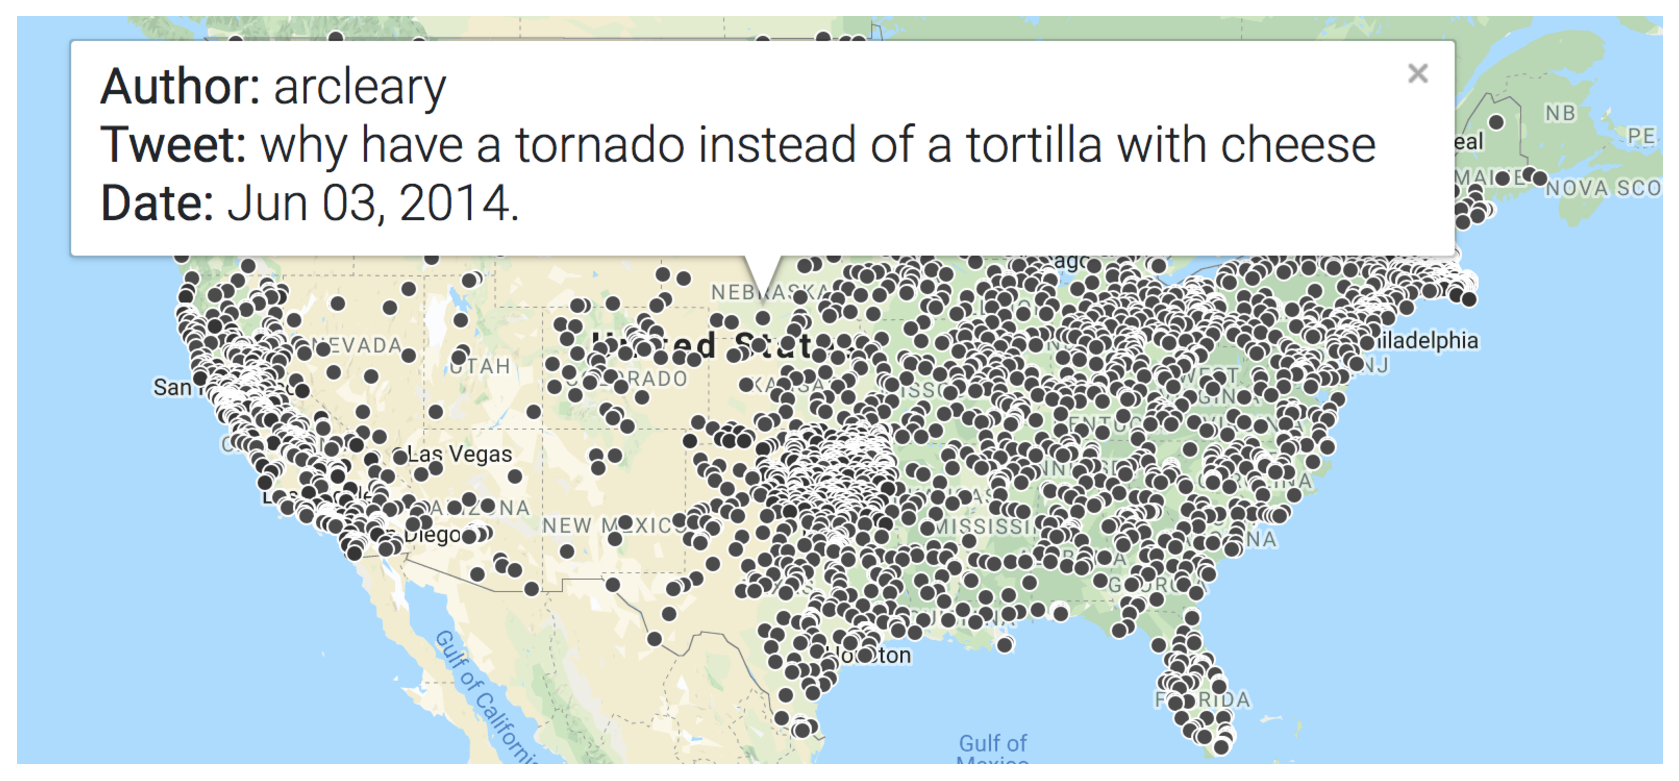
\includegraphics[width=4.07cm]{imgs/baseline.eps}\label{Fig:GlobalDisplay}}\hspace{0.05cm}\subfigure[Visually clustered results display.]{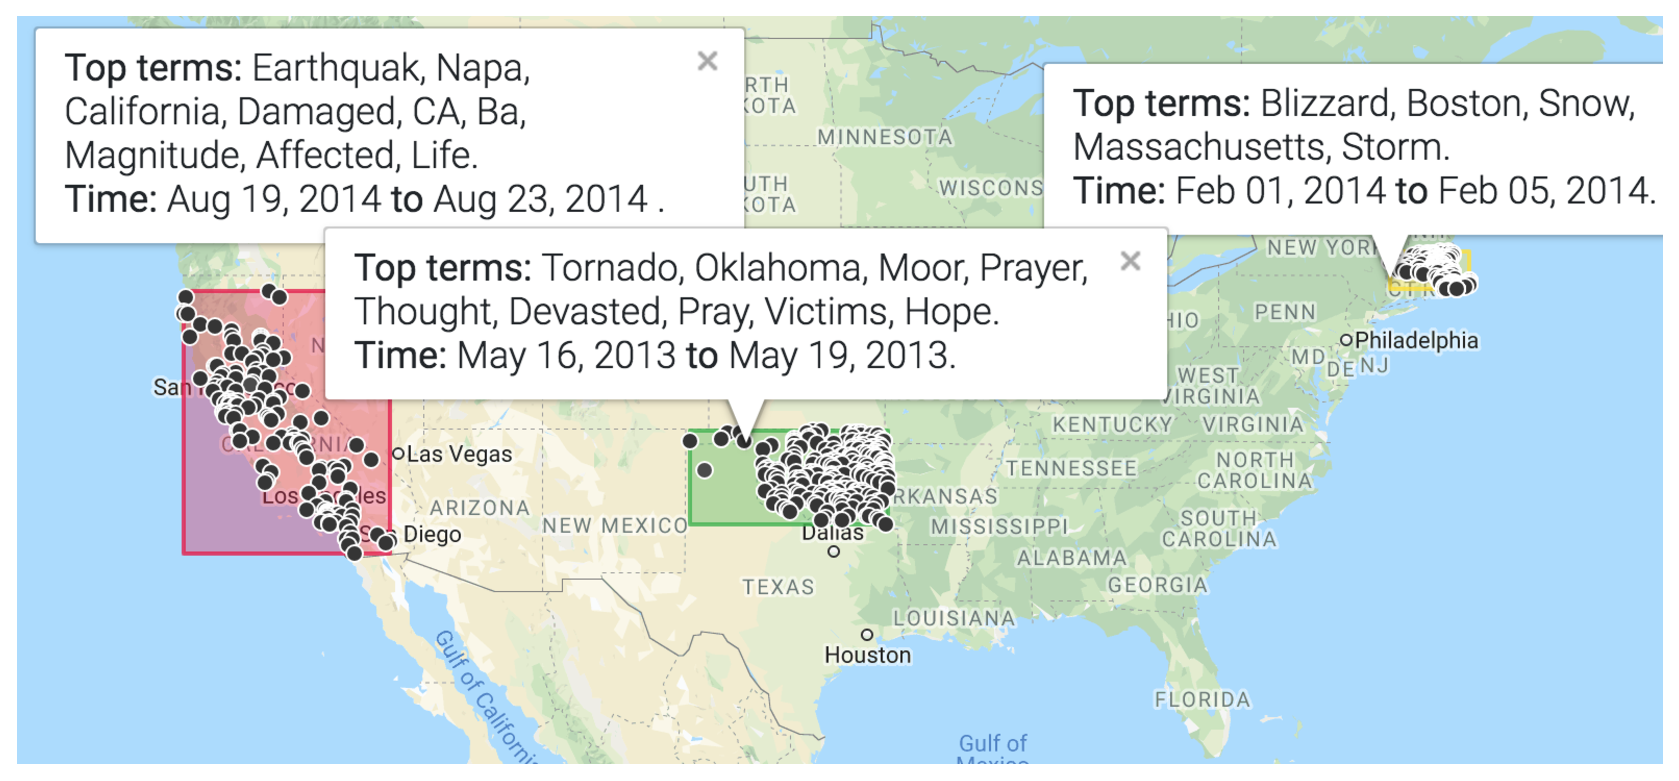
\includegraphics[width=4.07cm]{imgs/bps.eps}\label{Fig:FilteredDisplay}}
\par\end{centering}
\caption{(a) An interface for visual information retrieval showing all geolocated tweets that match a query related to natural disasters in a multiyear Twitter corpus, where \emph{all} matching tweets are shown.
%the query ``tornado, blizzard, earthquake''. 
(b) A clustered version of the same search results showing three clusters (i.e., bounding boxes) of tweets, in this case corresponding to three well-defined natural disasters: (i) a blizzard in Boston in February 2014, (ii) a tornado in Oklahoma in May 2013, and (iii) an earthquake in California in August 2014.  %In this paper we address how to maximize relevance and coverage of spatially, temporally, and contextually coherent clusters w.r.t.\ a  query through an optimization-based approach.
}
\label{Fig:UseCase}
\end{figure}

% \begin{table*}[t]
% \caption{Comparison between conventional Web Search and Filtering for AUIs.}
% \label{tbl:Comparaison2IR}
% \centering{}%
% \begin{tabular}{|c|>{\centering}p{6cm}|>{\centering}p{6cm}|}
% \hline 
%  & \textbf{Web Search} & \textbf{Filtering for AUIs}\tabularnewline
% \hline 
% \hline 
% \textbf{Information Need} & Realized by query  & Selection of an event or alert\tabularnewline
% \hline 
% \textbf{Form of Results} & Ranked list of documents & Filter settings (bounding box in visual display, time ranges, property
% filters) that select a subset of information elements to display\tabularnewline
% \hline 
% \textbf{Relevance Scoring} & Comparison of query and document content (and other relevant information)
% to generate a relevance score, e.g., via TF-IDF or BM25 & Third party application-specific tool (e.g., a machine learning approach)
% that predicts the probability that each information element is relevant
% to the selected alert\tabularnewline
% \hline 
% \textbf{Test Data for Benchmarking} & A set of queries; human-labeled judgments of document relevance to
% each query for a test corpus (i.e., ground truth relevance) & A set of alerts or events; human-labeled judgments of information element relevance
% to a selected alert (i.e., ground truth relevance)\tabularnewline
% \hline 
% \textbf{Evaluation} & Ranking metrics (P@k, AP, etc.) over documents given ground truth
% relevance  & Boolean metrics (e.g., F1-score) and Ranking metrics (P@k, AP, etc.)
% over information elements selected by the filter given ground truth
% relevance \tabularnewline
% \hline 
% \end{tabular}
% \end{table*}

To make the task of clustering in visual information retrieval more concrete, we introduce an example scenario.
Consider the case of searching a multiyear Twitter corpus for content related to natural disasters.  
% tornado, blizzard, earthquake
As shown in Figure~\ref{Fig:GlobalDisplay}, a typical visual approach would be to provide all matching tweets in an interactive visual interface.
%We denote all displayed content (in this case individual tweets)
%(such as user IP address, Tweet content, Tweet time, geographical coordinates, recent activity details) 
%as an information element that could
%be optionally shown or not.  
Clearly in this case, displaying all matching tweets simultaneously
results in a saturated and unreadable display that will take the user a large amount of time to sift through. 
To ease the task of browsing search results, a clustered results display like that shown in Figure~\ref{Fig:FilteredDisplay} can be used to restrict the displayed information to highly relevant clusters that cover a large fraction of relevant content. 
%Since results in clustering-based visual information retrieval interfaces are not individually selected, 
Hence it is critically important to define a clustering objective that optimizes for relevance, coverage, and visually coherent presentation of the clustered search results. %, which is the focus of this paper.

To the best of our knowledge, Viz-TIR is the first tool to address
relevance-driven clustering of search results in Visual Information Displays for social media, and moreover, to do so as the direct optimization of spatial, temporal, and content-based cluster parameters w.r.t.\ surrogates of F1-Score to balance cluster precision and recall.

% The contributions of this paper are summarized as follows: 
%  \begin{enumerate}
% \item We propose a new theory of IR for adaptive visual user interfaces. 
% \item We propose new expected metrics for optimization based on conventional IR metrics, i.e., precision, recall, and F1-Score.
% We argue that F1-Score and hence expected F1-Score is a good metric for this domain.
% \item We propose new filter setting search algorithms based on greedy strategies and optimal solutions. These algorithms are based on the optimization of new proposed metrics.
% %\item  We propose new MILP-based search method, which can also used about justification of new search algorithm.
% \item We present a thorough evaluation on three different datasets to show that the greedy algorithms we propose are a good approximation of the optimal method, and perform well in the presence of noise (i.e., corruption of the ground truth labels).
% %can even perform better with a noisy classifier \textendash{} up to 42\% improvement for a classifier with an accuracy of 60\%. On the other hand, 
% We experimentally demonstrate that the expected F1-Score metric is a good surrogate of F1-Score.
% %specifically with a highly accurate classifier \textendash{} for a classifier with 90\% accuracy, the RMSE is roughly 0.0111).
% \end{enumerate}

\section{V\texorpdfstring{\lowercase{iz}}-TIR Core Description}
In this section, we first define the mathematical notation used in this paper, then we proceed to propose Expected F1-Score (EF1) as a clustering objective well-suited to our task.  Finally, we briefly describe a fast greedy relevance-driven clustering algorithm for optimizing EF1 that drives our real-time Viz-TIR interface.


\subsection{Mathematical Notation}
Throughout this paper we use  the following mathematical notation:

\begin{itemize}
\item An tweet $j$ has three types of associated metadata: (i) textual content, which is composed of a set of terms of size $n$, (ii) a timestamp $t_e$, which may represent the creation date of $j$, and (iii) a position coordinates $(x_{e},y_{e})$.
\item Three variables $I(j)$, $B(j)$ and $S(j)$ are associated with each tweet $j$: $I(j)$ refers to whether a tweet $j$ is selected; $B(j)$ is a Boolean random variable indicating the relevance of a tweet $j$; $S(j)$ is a probabilistic score indicating the relevance of a tweet $j$ w.r.t. a query. 
$B(j)$ follows a \emph{Bernoulli} distribution with parameter $S(j)$, and hence, the expectation of $B(j)$ is $S(j)$, i.e., $\mathbb{E_S}[B(j)] = S(j)$.
  
\item $GC$ is the global set of tweets with total size $|GC|=m$. 

\item The set of tweets selected to match a user query is labeled $E$ with $E \subseteq  GC$; we use $E^*$ to refer to further subsets of tweets of clusters, i.e., $E^*\subseteq E$. 
Note that the size of $E$ can be represented as the sum of $I(j)$ among the global collection $GC$. Therefore, we have $|E| = \sum_{j=1}^m I(j)$.
\item We label the set of ground truth relevant tweets as the relevant set $RS$ consisting of $|RS|$ elements. 
Note that $|RS|$ is equal to the sum of $B(j)$ among the global collection $GC$. Therefore, we have $|RS| = \sum_{j=1}^m B(j)$.

\end{itemize}






\subsection{Deriving Expected F1-Score (EF1)}

We adopt the Boolean relevance framework standard in information retrieval~\cite{Baeza-Yates2010}. Thus, we assume that any information element $j$ has a ground truth relevance assessment $B(j)$ available at evaluation time.  
Because clusters are equivalent to Boolean retrieval (they either select or do not select elements) and we have a probabilistic estimate of relevance $S(j)$, we propose to evaluate
\emph{expected} variants of standard precision, recall, and F1-score.
While both precision and recall can be trivially optimized through pathological solutions (maximizing recall would select all information elements while maximizing precision would select the single highest probability information element), expected F1-score is a non-pathological objective that balances both expected precision and recall. % in a Boolean retrieval framework.

Recalling our previous definitions, given a set of selected information elements  $E$ and a relevant set $RS$, %the global information element collection $GC$ with size $m$, 
by rearranging and cancelling terms, the F1-Score of $E$ can be expressed as follows:
\begin{equation}
   F1(E)=\dfrac{2\times\sum_{j\in E}B(j)}{|E|+|RS|}= \fbox{$ \dfrac{2\times\sum_{j=1}^{m}B(j)I(j)}{\sum_{j=1}^{m}I(j)+\sum_{j=1}^{m}B(j)}$}
\end{equation}

 
Taking a 1st order Taylor expansion, we have the following expectation approximation 
$\mathbb{E}(X/Y)\approx \mathbb{E}(X)/ \mathbb{E}(Y)$ for two dependent random variables $X$ and $Y$~\cite{Kempen2000}. Hence, given that $B(j)$ is a Boolean random variable, we define an \emph{approximated expected recall} as: 
\begin{equation}
\mathit{EF1}(E)=\mathbb{E_{S}}\left[\Box\right]\approx\dfrac{2\times{\displaystyle \sum_{j=1}^{m}}\mathbb{E_{S}}[B(j)]I(j)}{{\displaystyle \sum_{j=1}^{m}}I(j)+\sum_{j=1}^{m}\mathbb{E_{S}}[B(j)]}=\dfrac{2\times{\displaystyle \sum_{j=1}^{m}}S(j)I(j)}{{\displaystyle \sum_{j=1}^{m}}I(j)+{\displaystyle \sum_{j=1}^{m}}S(j)}
\end{equation}



\subsection{Greedy relevance-driven clustering}
Now we greedily optimize $\mathit{EF1}(E)$. 
In this work, we assume that three types of clustering ``parameters'' are used to optimize clusters: Keywords, Time, and Space.  A cluster is generated by \emph{conjoining} these three selection parameters. In the following, we describe how to greedily optimize each of these selection parameters by iterative pruning, how to combine them for producing relevance-driven clusters, and finally, how to generate multiple relevant clusters.

\subsubsection{Greedy Keyword Selection algorithm}

Given a set of information elements matching a user query, the Greedy Keyword Selection algorithm aims to select a set of keywords  in order to exclude a subset of tweets containing these keywords for the purpose of maximizing the EF1-Score. 
Formally, the algorithm aims to select an
optimal subset of $k$ terms $T_{k}^{*}\subset T_E$ (where $|T_{k}^{*}|=k$ and $T_E$ are terms of the initial set of elements) to exclude tweets containing these keywords for optimizing the EF1-score. This is achieved by
building $T_{k}^{*}$ in a greedy manner by choosing the next optimal
term $t_{k}^{*}$ given the previous set of optimal term selections
$T_{k-1}^{*}=\{t_{1}^{*},\ldots,t_{k-1}^{*}\}$ (with $T_{0}^{*}=\emptyset$)
using the following criterion:
\begin{equation}
t_{k}^{*}=\argmax_{t_{k}\notin T_{k-1}^{*}}\hspace{-0.3mm}[EF1(E^{*} \textrm{ that don't contain } \{t_{1}^{*},\dots t_{k}^{*}\})]
\end{equation}
where  $E^{*}$ is a subset of the initial tweet set $E$ that don't contain the keywords $\{t_{1}^{*},\dots t_{k}^{*}\}$. 


\subsubsection{Greedy Time Selection algorithm}

The idea behind the time-based greedy selection algorithm is as simple as finding a time window range $[t_{start},t_{end}]$ for \emph{temporal coherency} of clusters, which allows to select a subset of tweets $E^{*}\subseteq E$ falling in that time window, with $E^{*}$ having the highest EF1-Score. 
Formally, given a list of elements $E=\{j_{t_1}\leq \dots \leq j_{t_n}\}$, where "$\leq$" specifies the timestamp order, we propose to use \emph{binary partitioning search} (BPS) to find the best set that optimizes EF1.


\begin{figure*}[t]
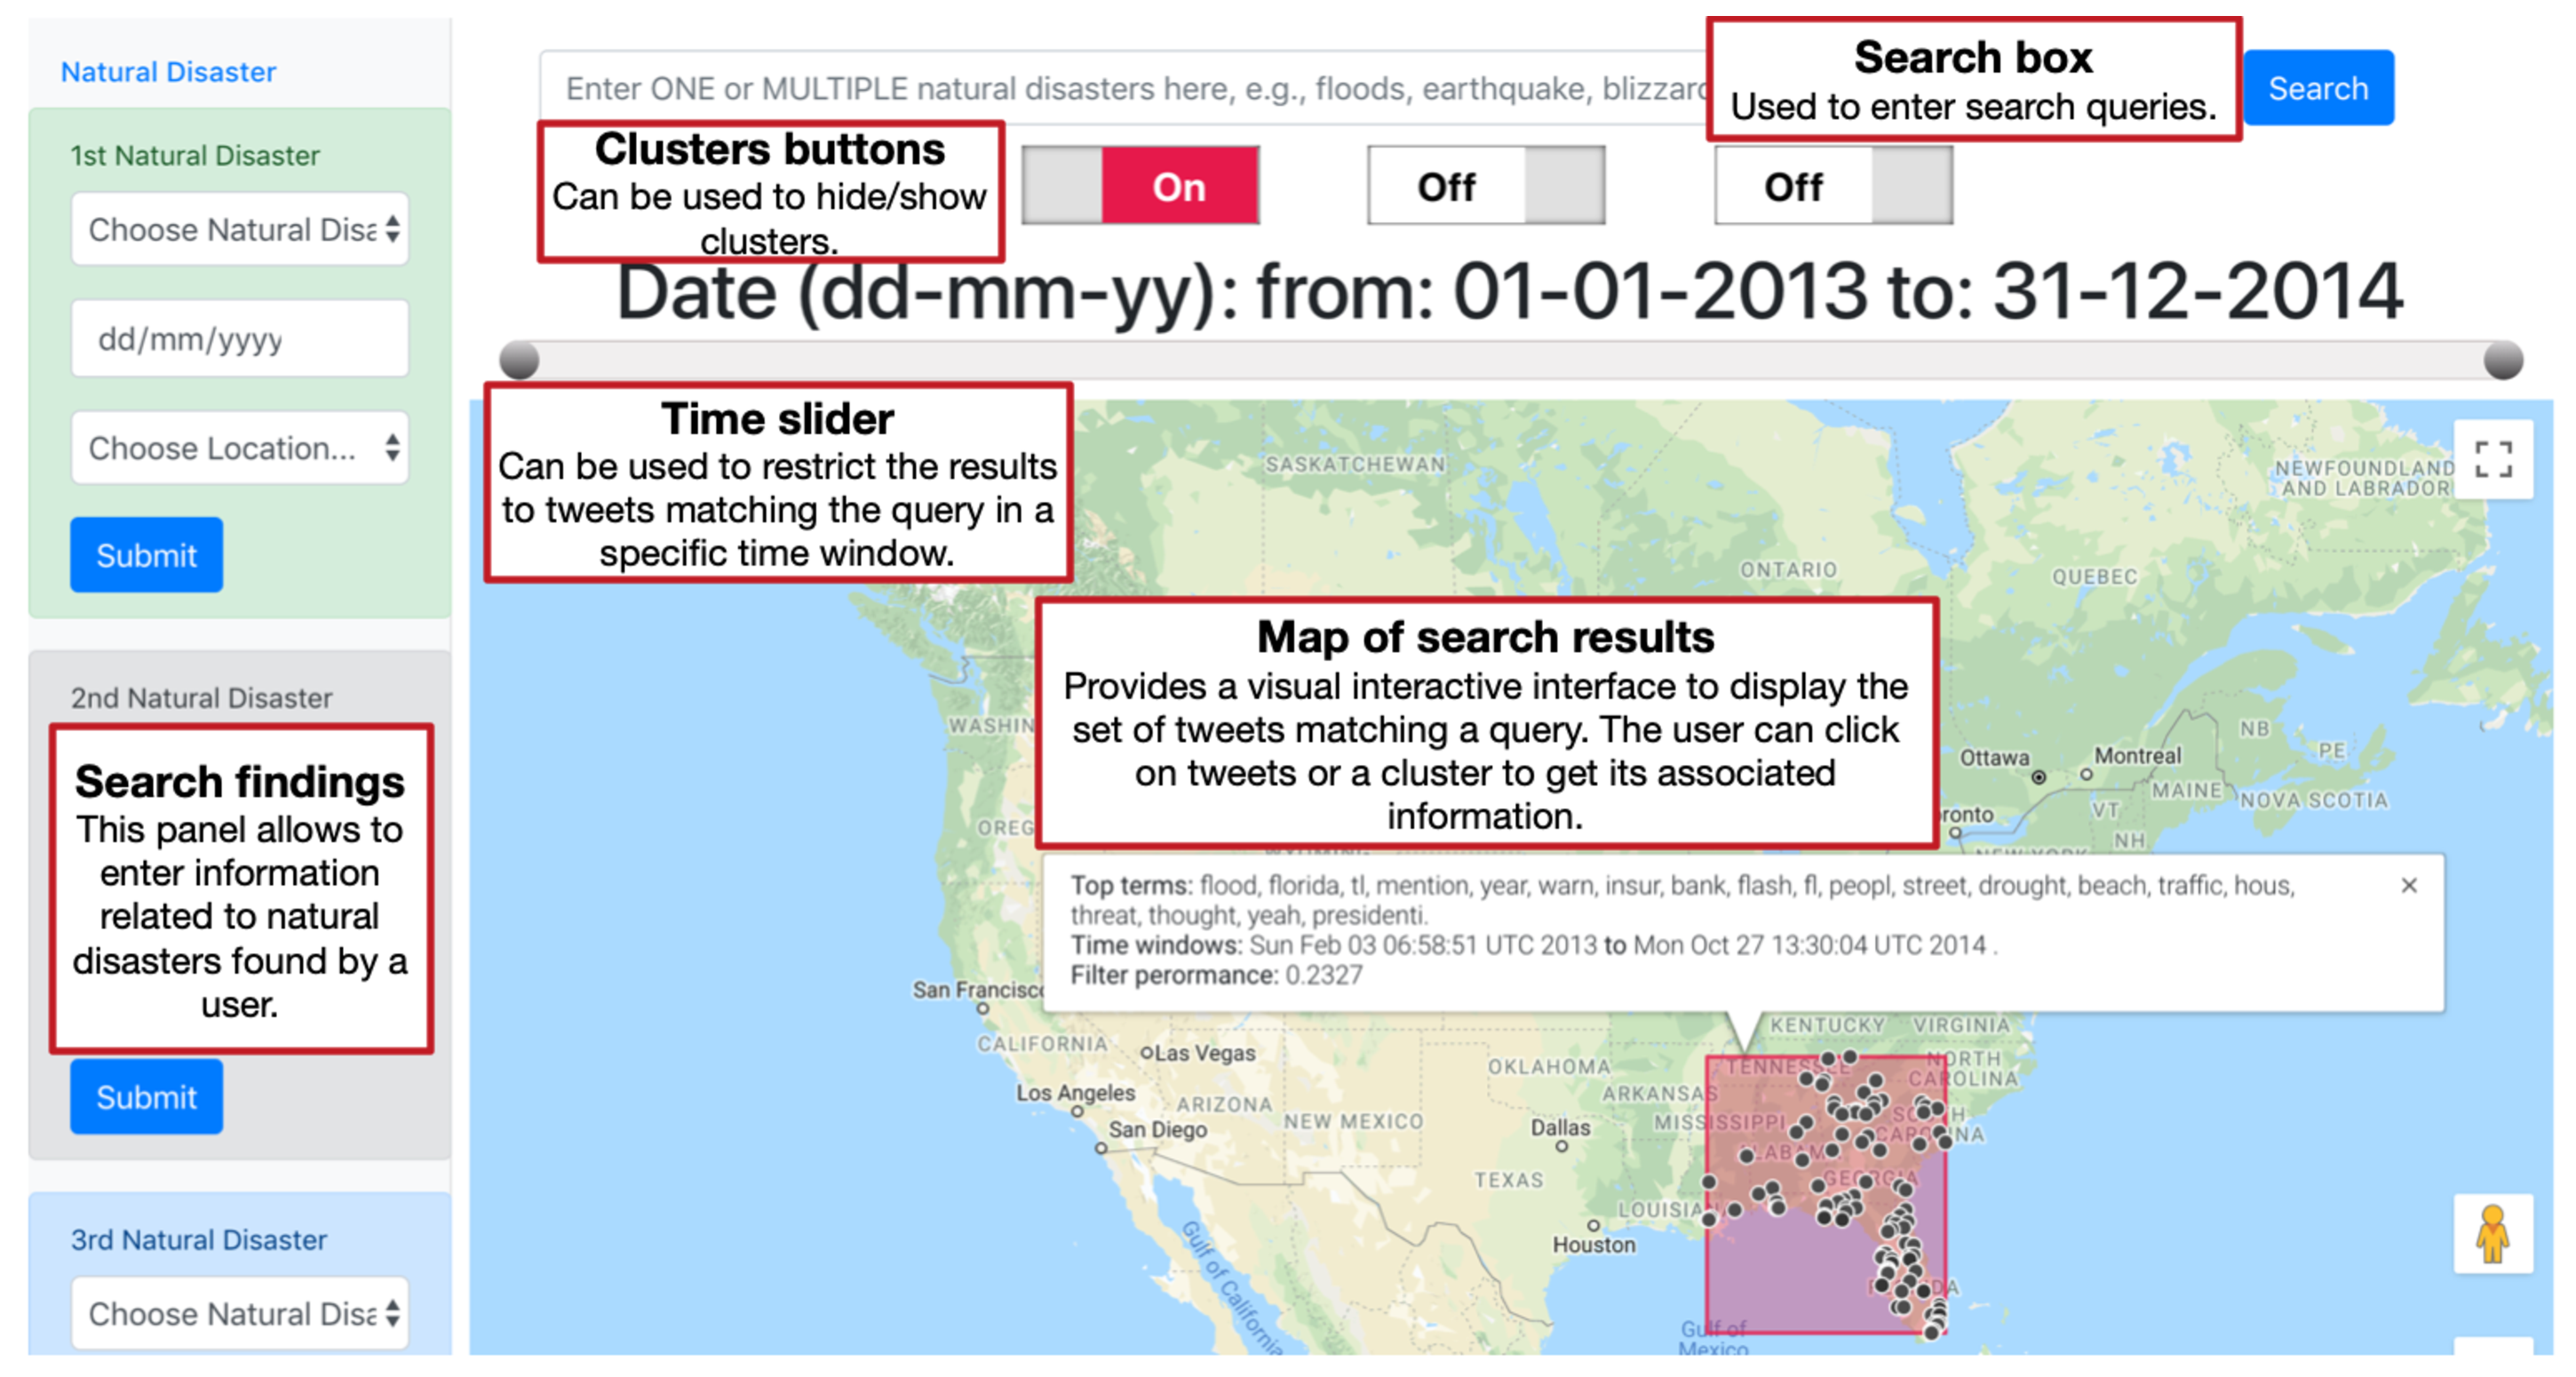
\includegraphics[width=15cm]{imgs/main.eps}
\caption{Main interface of the demonstration.}
\label{fig:MainInterface}
\end{figure*}


\subsubsection{Greedy Spatial Selection algorithm}

It is critical to main \emph{visual coherency} of clusters and bounding boxes are one way to visually bound regions that facilitate direct optimization.
The aim of the spatial greedy selection algorithm is to return coordinates $[(x_{min},y_{min}),(x_{max},y_{max})]$ representing the EF1-Score maximizing bounding box represented by the lower and upper bound coordinates -- respectively $(x_{min},y_{min})$ and $(x_{max},y_{max})$. This 2D problem is similar to the previous one dimensional problem of finding the best time window. Therefore, we propose to sequentially apply a BPS on the x-axis to determine $(x_{min},x_{max})$, then on the y-axis to determine $(y_{min},y_{max})$. 



\subsubsection{Relevance-driven clustering algorithm} To obtain a cluster combining the above selection parameters, we propose a greedy algorithm, which at each iteration applies all the above selection algorithms and chooses the one that improves the most EF1.  The selected cluster is updated with its new setting and the iteration continues.  Iterations terminate when no selection algorithm can unilaterally improve EF1 and the final cluster is returned.


\subsubsection{Multiple Cluster Selection Wrapper}

In practice a single cluster chosen by the previously described algorithm will narrow the user in a single \textquotedblleft information perspective\textquotedblright{}. However, there will likely be multiple perspectives and so the user should have a choice of multiple clusters.  
Consider Figure~\ref{Fig:UseCase}: this actually shows three different spatial bounding boxes corresponding to three different events provided by three clusters.
Here, we provide a greedy approach for providing a ranked list of clusters. 
The algorithm itself is quite simple: after the first cluster is produced, all selected tweets in that cluster have their scores $S(j)$ zeroed out.  The relevance-driven clustering algorithm is then run again, where it will inherently focus on a different content set.  



% Not sure how critical this is (and we need space) -Scott
%Viz-TIF is built on the top of the Lucene IR system\footnote{\url{https://lucene.apache.org/core/}} for the indexing, query processing and retrieval part, and on the Google Maps API for data visualization.

\section{Demonstration Overview}


The demonstration will be illustrated using a scenario related to  finding natural disasters discussed in a collection of tweets.  
We used Twitter data crawled
using the Twitter Streaming API for two years spanning 2013 and 2014~\cite{Iman2017} with the following restrictions intended for user experimentation:
(i)~the dataset was restricted to users located within the US, (ii)~non-English tweets were filtered out, (iii)~only the tweets related to 12 natural disasters were kept -- tweets related to other natural disasters were removed. These natural disasters are temporally, and geographically disjoint -- a storm, a hurricane,  a drought, two floods, two earthquakes, two tornadoes,  and three blizzards. Finally, (iv)~false positive tweets mentioning natural disaster keywords but not related to a particular natural disaster were intentionally included. The final dataset contains 39,486 tweets with 5,075 relevant natural disaster tweets.


As shown in Figure~\ref{fig:MainInterface}, the demonstration's main user interface allows users to enter a search query with search results then shown on an interactive map used to browse the results. The user can interact with the map by panning and zooming and also by clicking on tweets and clusters to view their content (for clusters, we display a summary in terms of selected keywords). Also, the user will be able to use a time slider bar to restrict the results to tweets in a specific time window. 

In the scenario of this demonstration, the user will experience finding three different natural disasters using three different algorithms.
In addition to Viz-TIR, two different algorithms are used to show the effectiveness of Viz-TIR, including: (i) a baseline method which displays all tweets that match a query (see Figure~\ref{fig:main2}) and (ii) X-Means~\cite{Pelleg2000} (an extension of $k$-means, which tries to  automatically determine the number of clusters) -- a baseline method for clustering the top relevant results (see Figure~\ref{fig:xmeans}).  
At each step, the user will be asked to enter information related to each natural disaster they may identify, including the type of the natural disaster, its location (US state), and the date on which they think the disaster first occurred.

In this demonstration, a user can perform interactive searches such as the following example search scenarios:

\subfour{Baseline scenario:} A user may search for information on natural disaster events. Using the query box, the user enters the keyword ``earthquake''. As shown in Figure~\ref{fig:main2}, the baseline algorithm shows all tweets that match the query on the map using circles with a color range corresponding to the probability of relevance.
% [Following parts not critical and we need the space.]  -Scott
%-- light gray circles represent low probability relevance tweets, and dark gray circles represent high probability relevance tweets.


\begin{figure}[H]
\begin{centering}
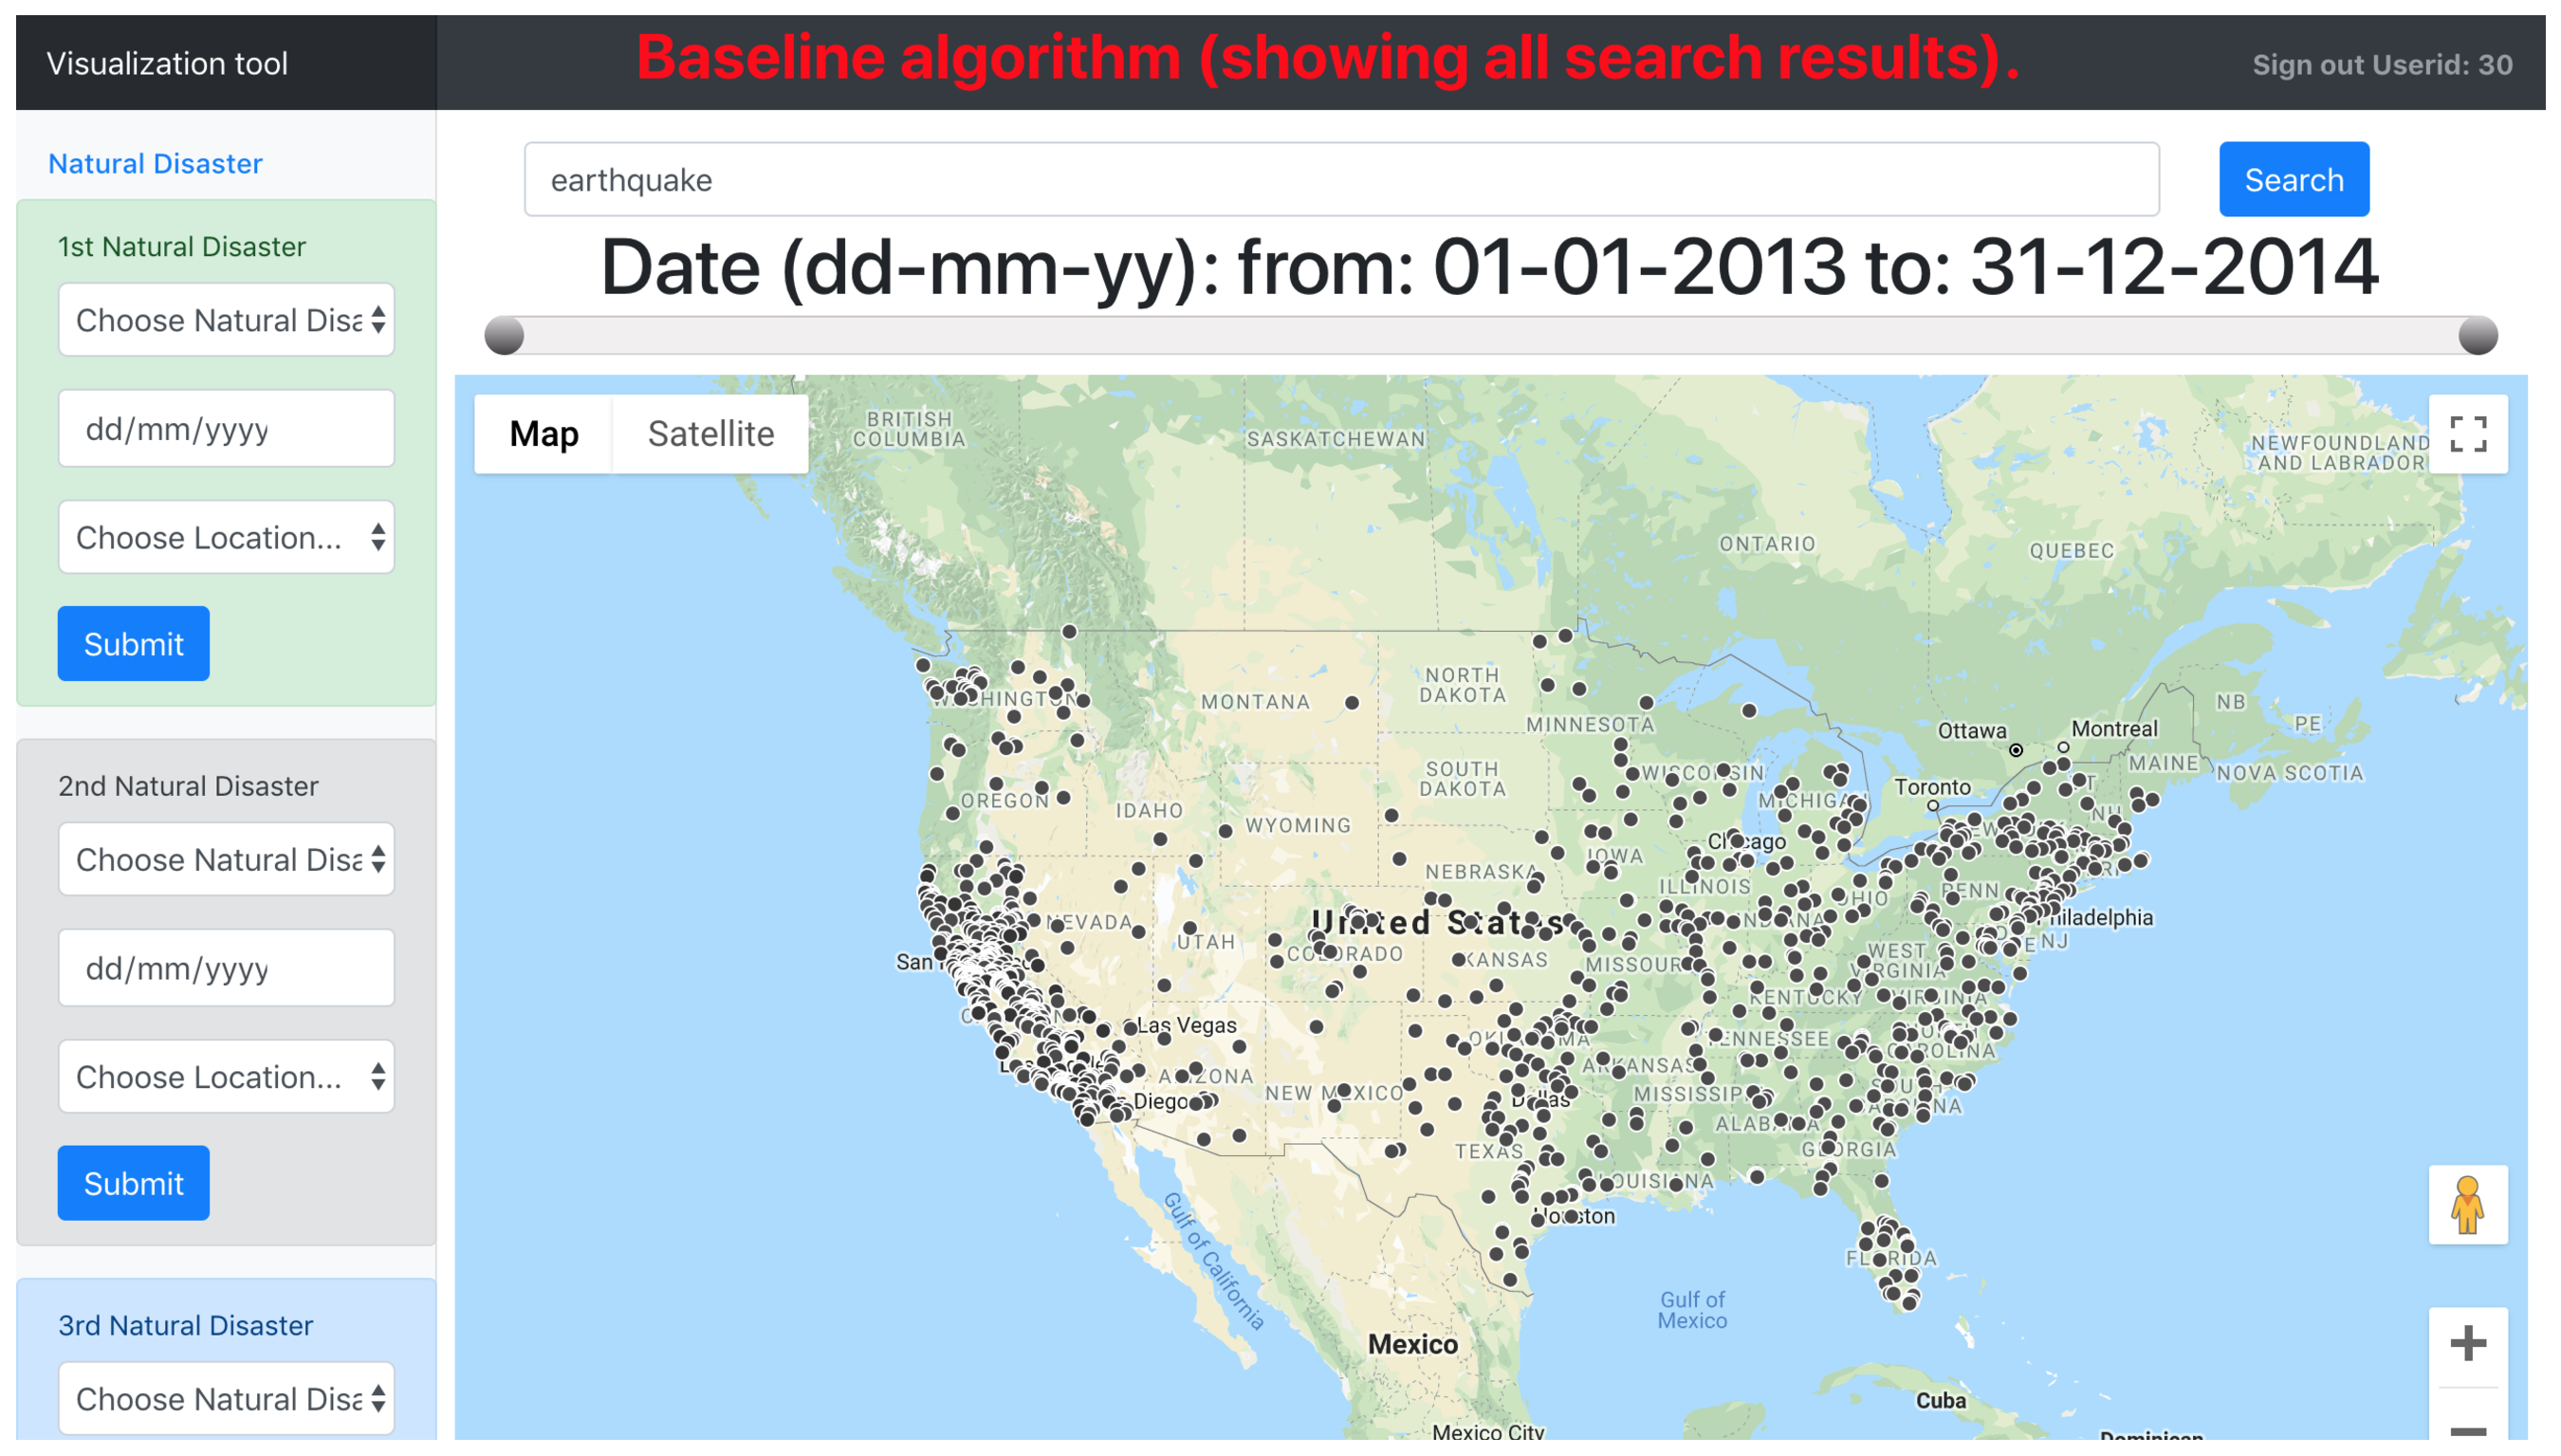
\includegraphics[width=6.25cm]{imgs/baseline1.eps}
\par\end{centering}
\caption{All results that match the query.}
\label{fig:main2}
\end{figure}

\noindent As shown in Figure~\ref{fig:main3}, the user can restrict the list of tweets shown to a specific time window with the time slider; here a cluster of tweets appears indicating an earthquake in California during August 2014. The user may click on tweets to learn more about that event.
% [Following parts not critical and we need the space.]  -Scott
%in order to fill the sidebar with the appropriate information. The user may then proceed to search other natural disasters in a similar manner.

\begin{figure}[H]
\begin{centering}
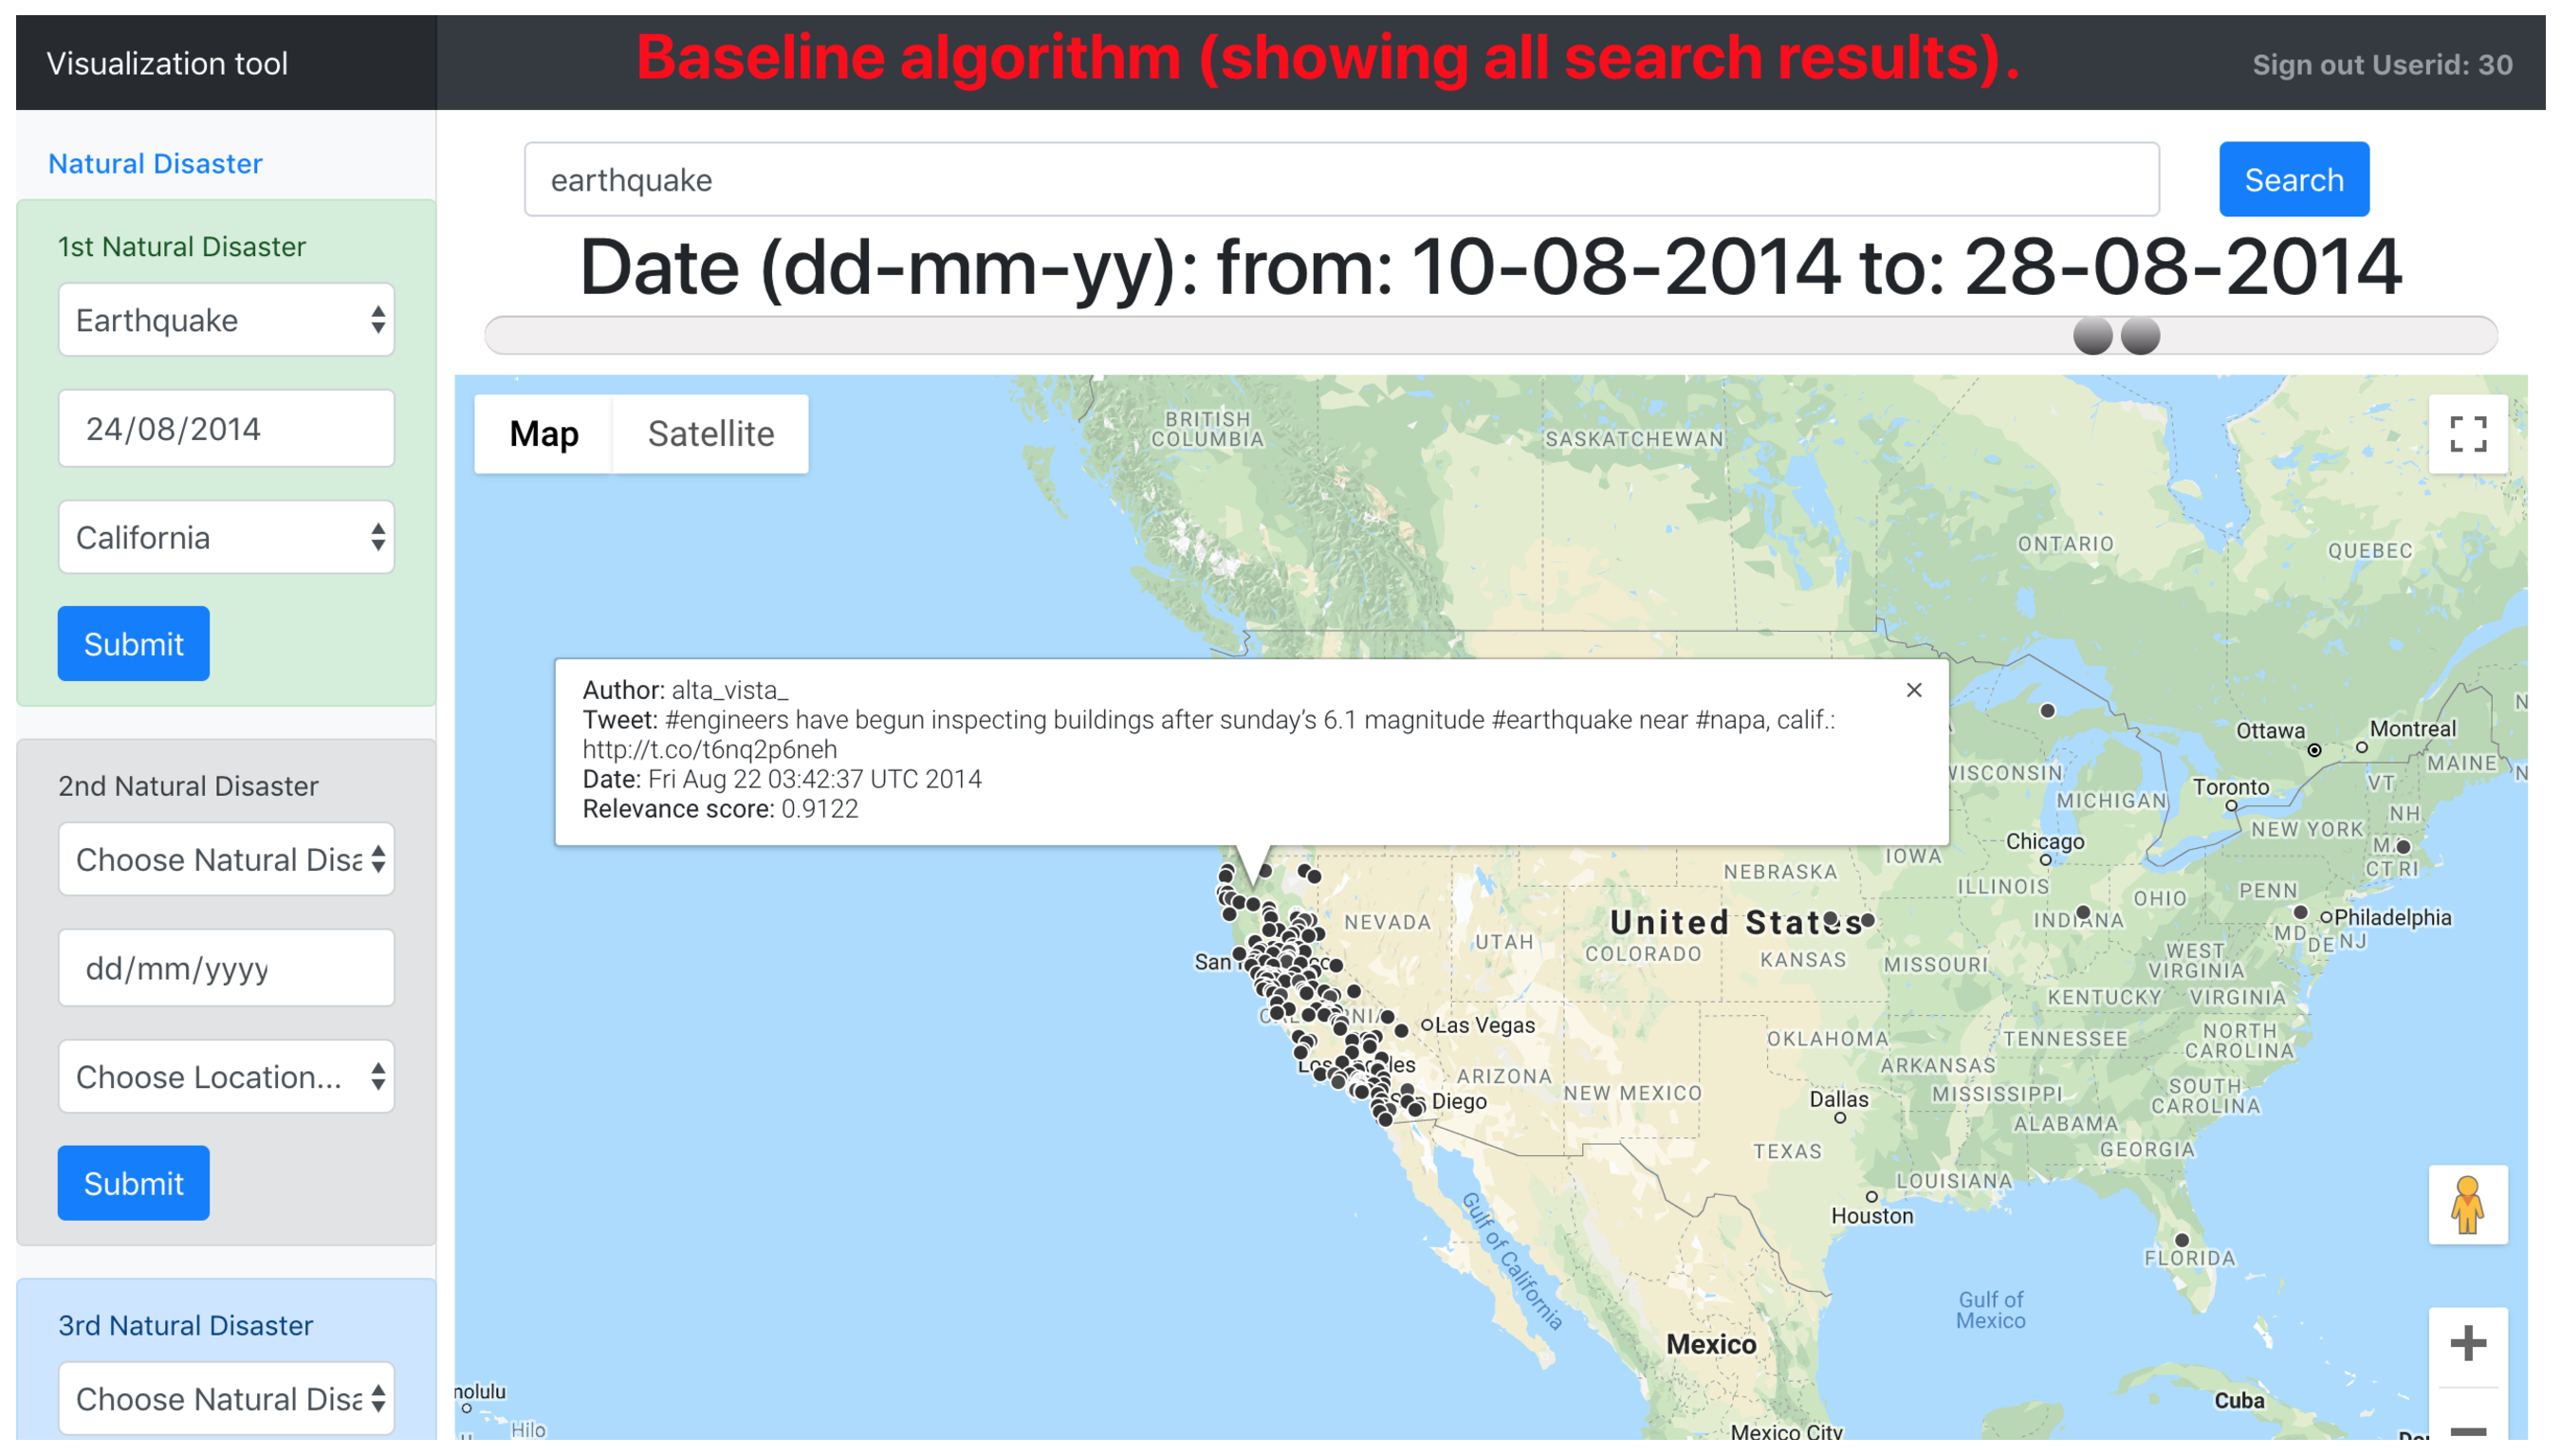
\includegraphics[width=6.25cm]{imgs/baseline2.eps}
\par\end{centering}
\caption{Sub-set of the results that match the query.}
\label{fig:main3}
\end{figure}


\subfour{Clustering scenarios:} 
The scenario using $k$-means or EF1 is similar. For example, the user may search multiple natural disasters using the multi-term query ``earthquake, blizzard, tornado''. As shown in Figures~\ref{fig:xmeans} and~\ref{fig:bps2}, clusters will appear for both algorithms, which show different clustered information perspectives.
% [Following parts not critical and we need the space.]  -Scott
%The user may, for example, decide the show only the top 3 clusters for a more efficient investigation. 
The user can then click on a cluster to get a summary description.
%sense of the event represented by the cluster, including top terms, and event time window. 
% Not critical for the demo description -- unclear why we mention this so just exclude.  -Scott
%Again, once the user thinks that he has identified a natural disaster, he will have to enter its related information into the sidebar.

\begin{figure}[H]
\begin{centering}
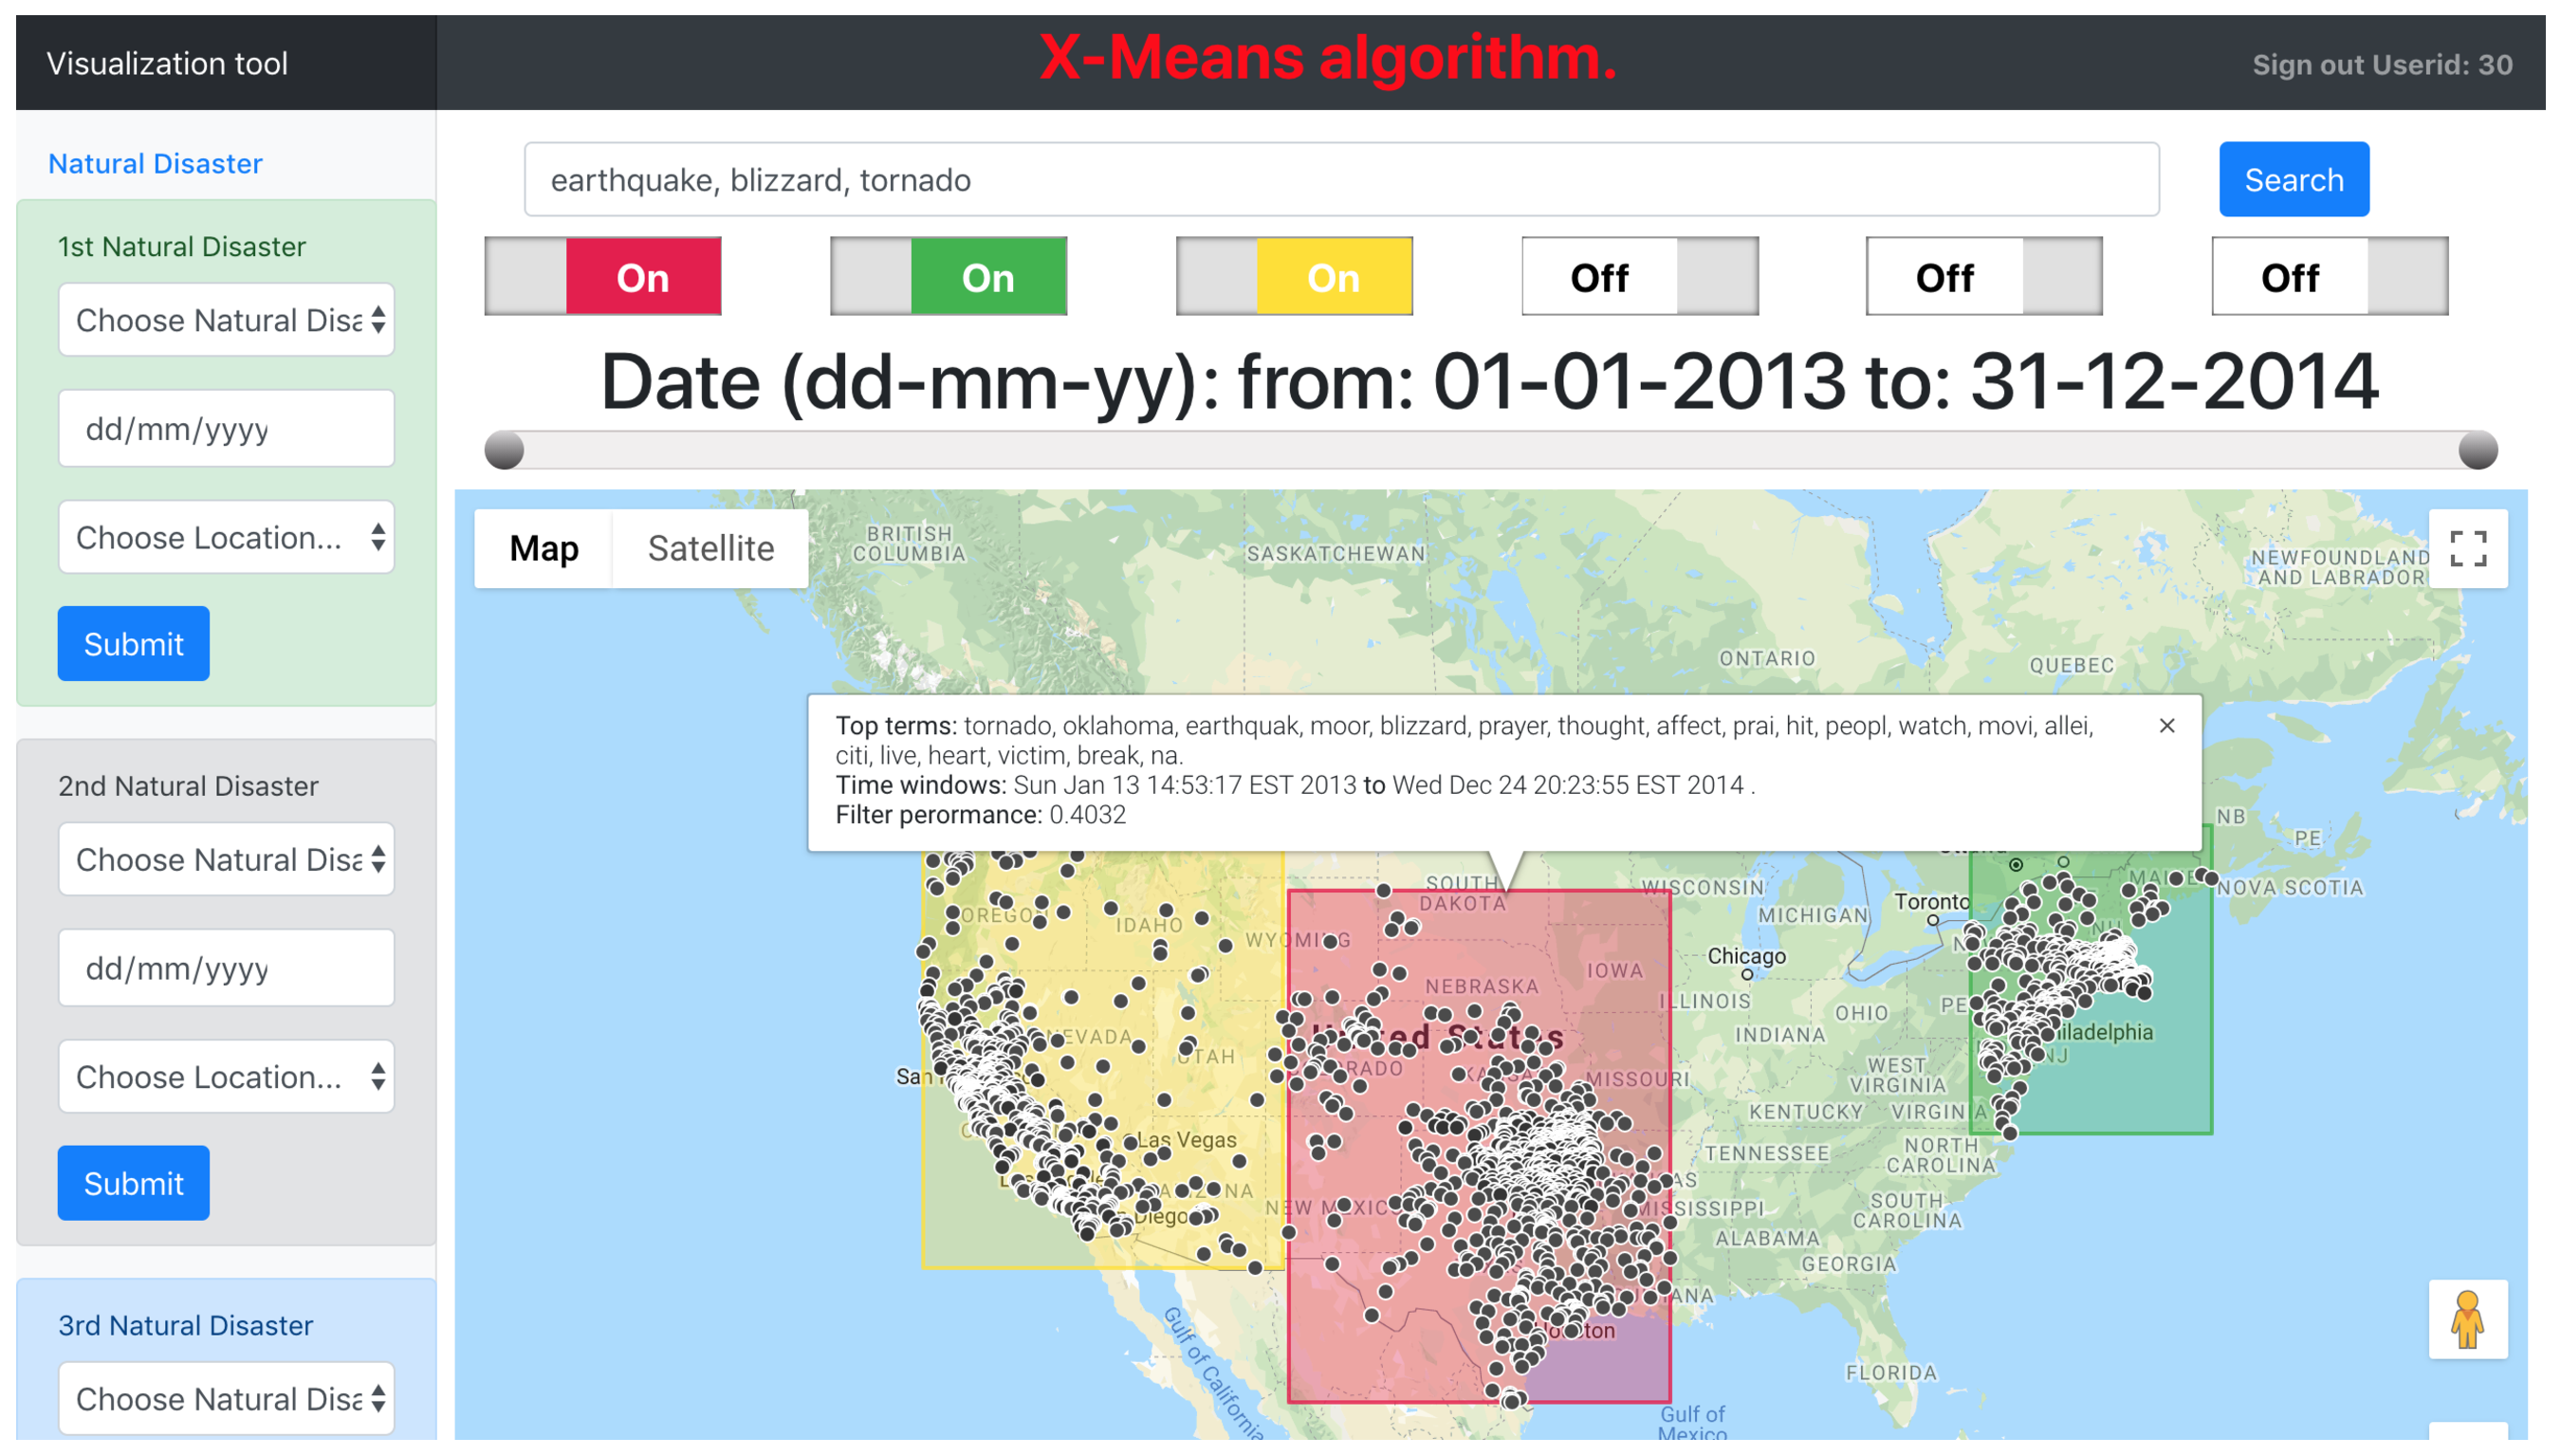
\includegraphics[width=6.25cm]{imgs/x-means.eps}
\par\end{centering}
\caption{Clustered results using X-Means.}
\label{fig:xmeans}
\end{figure}

\begin{figure}[t]
\begin{centering}
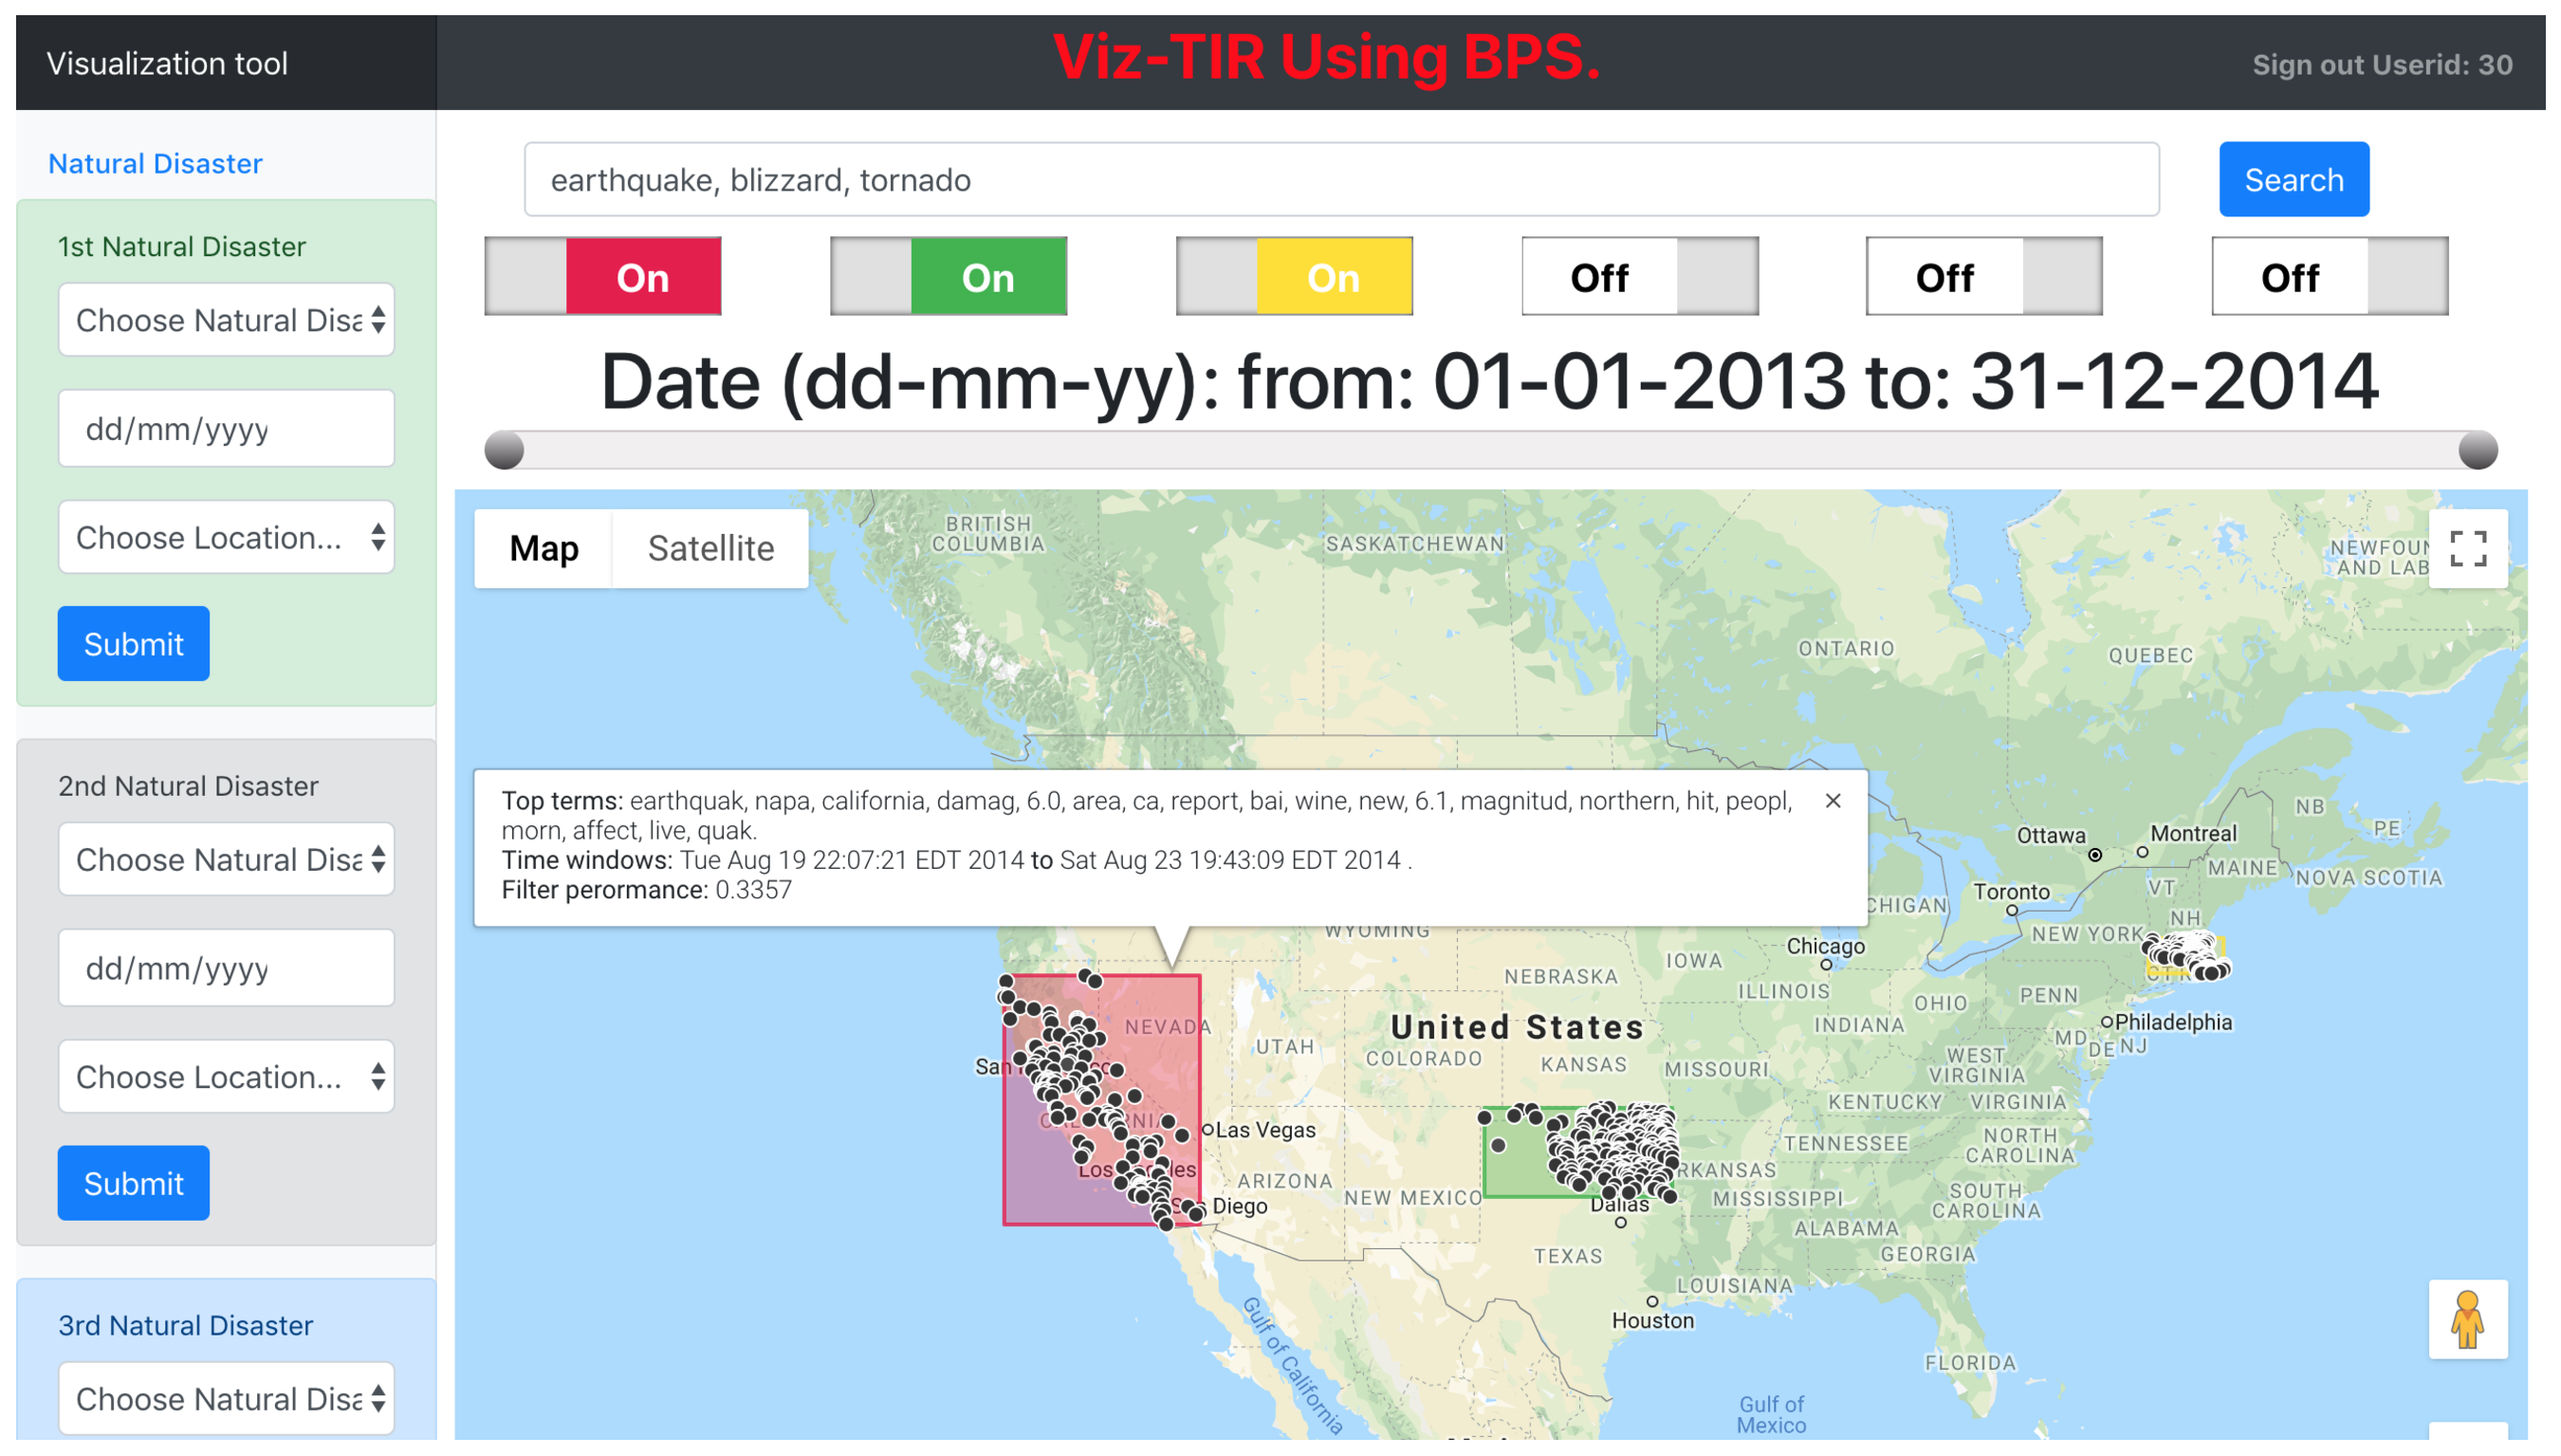
\includegraphics[width=6.25cm]{imgs/bps2.eps}
\par\end{centering}
\caption{Compact clustered results using EF1 (Viz-TIR).}
\label{fig:bps2}
\end{figure}

\begin{figure}[t]
\begin{centering}

\includegraphics[width=7.5cm]{imgs/legend9.eps}
\par\end{centering}
\begin{centering}
{\includegraphics[width=8.5cm]{imgs/nd_recall.eps}}
\par\end{centering}
\caption{The performance of the algorithms measured using cumulative recall for the type and location of the natural disasters and the absolute error in the dates of the disasters.}
\label{fig:UserSurveyRecall}
\end{figure}

\subfour{User Study:} 
To determine whether our proposed relevance-driven EF1 optimization approach to clustering improves human search task performance in the Viz-TIR visual search interface (in comparison to $k$-means clustering and the non-clustering baseline), we performed an evaluation of 24 users who were given the task of searching for natural disasters in the previously described data.  An analysis of their performance is provided in Figure~\ref{fig:UserSurveyRecall}, which shows that on average, users have higher recall on natural disaster 
types and locations as well as lower error estimating the time of the disaster using EF1 clustering in comparison to other methods.
% Insert Figure 4 from
% https://www.overleaf.com/20402227yvddjdhgzbcs#!#%2F73602764%2F

% [Specific experimental details below are not important.  We want to discuss the high-level ideas and big picture take-home points.]  -Scott
%Comparing the two clustering methods, we already noted in our previous user study that very often,  Viz-TIR provides more contextualized clusters with more precise locations and time windows around the true event than X-Means (As shown in Figures~\ref{fig:xmeans} and~\ref{fig:bps2}). This is due to the fact that Viz-TSF relies on a relevance-driven based clustering algorithm.
%At the end, the user will be shown a comparative performance of how well he was able to identify the natural disasters using the three algorithms.
%Finally, With the consent of participants to our demonstration, we also plan to collect logs and other survey information to enrich the current user study we are carrying out.

\section{Summary and Future Work}

In this paper, we have developed Viz-TIR, a tool to visually search Twitter content through spatial, temporal, and content-based clustering. Viz-TIR formulates clustering as a relevance-driven optimization problem 
%the probabilistic relevance estimate of tweets
w.r.t.\ a user-provided query.
In particular, Viz-TIR leverages a fast greedy optimization algorithm
to maximize an approximation of the expected F1-Score metric to generate multiple clusters for visual display. 
We provide a demonstration use case that compares Viz-TIR with two baselines over 2 years of Twitter content for finding information related to natural disasters.

Important areas of future work include consideration of the role of (pseudo-)relevance and other explicit or implicit feedback methods to create a tighter and more responsive user interaction loop. 
Furthermore, in combination with user studies and consideration of human factors, future work should also consider novel application-specific objectives, e.g., in specific visualization frameworks or based on a ranking theory of results presentation (e.g., using size or color for visual ranking emphasis).

%% ==================================================================

%In this paper we have introduced Viz-TIF, a tool to search Twitter
%content through spatial, temporal, and content-based filters to help
%focus the user's exploration of search results with geo-temporally
%coherent content.

%By treating filter selection for a user's queries as an expected F-Score optimization problem (as opposed to an unsupervised clustering problem that is unaware of visual presentation of filters, or query relevance estimates), Viz-TIR was able to select relevant filters to provide temporal, spatial, and keyword context for distinct events related to the user's queries.
% Also filters are custom-built for a given (visual) interface.  -Scott
% Get context with filters, don't get this with clustering.  -Scott
%We have described a specific search scenario of queries related to an information of natural disasters occurring in the US during a two year period and showed the capabilities of using Viz-TIF to search large-scale data in social networks.

%Overall, we aim for this work to bring a formal IR perspective to
%the important research area of AUIs while opening new research directions
%for the application of optimization techniques for filter selection
%in AUIs. As information retrieval has transformed our web experience,
%we believe there is a similar opportunity to transform the present
%nascent state of AUIs through optimization and information retrieval
%principles to make them more ubiquitous in our daily lives.  We hope this demonstration serves as one example of such a novel visual information retrieval interface.

\subfour{Acknowledgement:}
We would like to thank Yihao Du for running the user study.


\bibliographystyle{unsrt}
\balance
\bibliography{biblio}

\end{document}
